\chapter{QMainWindow}

QMainWindow 类用于创建主程序窗口。 更多内容...


\begin{tabular}{|r|l|}
	\hline
	属性 & 方法 \\
	\hline
	头文件 & \#include <QMainWindow>\\      
	\hline
	qmake & QT += widgets\\      
	\hline
	继承: &	QWidget\\
	\hline
\end{tabular}

\begin{compactitem}
\item 列出所有成员函数, 包括继承的成员函数
\end{compactitem}

\section{公共成员类型}

\begin{tabular}{|r|m{25em}|}
	\hline
	类型 & 方法 \\
	\hline
    enum &	DockOption \{ AnimatedDocks, AllowNestedDocks, AllowTabbedDocks, ForceTabbedDocks, VerticalTabs, GroupedDragging \} \\ 
    \hline
    flags &	DockOptions \\ 
	\hline
\end{tabular}

\section{属性}

\begin{tabular}{|r|l|}
	\hline
    属性名 &	类型 \\ 
    \hline
    animated 	& bool \\ 
    \hline
    dockNestingEnabled &	bool\\
    \hline
    dockOptions &	DockOptions\\
    \hline
    documentMode 	&bool\\
    \hline
    iconSize  &	QSize\\
    \hline
    tabShape 	&QTabWidget::TabShape\\
    \hline
    toolButtonStyle &	Qt::ToolButtonStyle\\
    \hline
    unifiedTitleAndToolBarOnMac &	bool\\
	\hline
\end{tabular}

\section{公共成员函数}

\begin{longtable}[l]{|r|m{20em}|}
\hline
返回类型  & 	函数名 \\
\hline
 &QMainWindow (QWidget *parent = nullptr, Qt::WindowFlags flags = Qt::WindowFlags()) \\ 
 \hline
virtual  &	$\sim$QMainWindow () \\
\hline
void 	&addDockWidget (Qt::DockWidgetArea area, QDockWidget *dockwidget) \\ 
\hline
void 	&addDockWidget (Qt::DockWidgetArea area, QDockWidget *dockwidget, Qt::Orientation orientation) \\
\hline
void 	&addToolBar (Qt::ToolBarArea area, QToolBar *toolbar) \\ 
\hline
void 	&addToolBar (QToolBar *toolbar) \\ 
\hline
QToolBar *& 	addToolBar (const QString \&title) \\
\hline
void 	&addToolBarBreak (Qt::ToolBarArea area = Qt::TopToolBarArea) \\
\hline
QWidget *& 	centralWidget () const \\ 
\hline
Qt::DockWidgetArea &	corner (Qt::Corner corner) const \\
\hline
virtual QMenu * &	createPopupMenu () \\
\hline
QMainWindow::DockOptions& 	dockOptions () const\\
\hline
Qt::DockWidgetArea 	&dockWidgetArea (QDockWidget *dockwidget) const\\
\hline
bool &	documentMode () const \\
\hline
QSize &	iconSize () const\\
\hline
void 	&insertToolBar (QToolBar *before, QToolBar *toolbar)\\
\hline
void 	&insertToolBarBreak (QToolBar *before)\\
\hline
bool 	&isAnimated () const\\
\hline
bool 	&isDockNestingEnabled () const\\
\hline
QMenuBar *& 	menuBar () const \\ 
\hline
QWidget * &	menuWidget () const \\ 
\hline
void 	&removeDockWidget (QDockWidget *dockwidget)\\ 
\hline
void 	&removeToolBar (QToolBar *toolbar) \\ 
\hline
void 	&removeToolBarBreak (QToolBar *before) \\ 
\hline
void 	&resizeDocks (const QList<QDockWidget *> \&docks, const QList<int> \&sizes, Qt::Orientation orientation) \\ 
\hline
bool 	&restoreDockWidget (QDockWidget *dockwidget) \\ 
\hline
bool 	&restoreState (const QByteArray \&state, int version = 0) \\ 
\hline
QByteArray &	saveState (int version = 0) const \\ 
\hline
void &	setCentralWidget (QWidget *widget) \\ 
\hline
void &	setCorner (Qt::Corner corner, Qt::DockWidgetArea area) \\ 
\hline
void 	&setDockOptions (QMainWindow::DockOptions options) \\ 
\hline
void &	setDocumentMode (bool enabled) \\ 
\hline
void &	setIconSize (const QSize \&iconSize) \\ 
\hline
void &	setMenuBar (QMenuBar *menuBar) \\ 
\hline
void& 	setMenuWidget (QWidget *menuBar) \\ 
\hline
void &	setStatusBar (QStatusBar *statusbar) \\ 
\hline
void &	setTabPosition (Qt::DockWidgetAreas areas, QTabWidget::TabPosition tabPosition) \\ 
\hline
void &	setTabShape (QTabWidget::TabShape tabShape) \\ 
\hline
void 	&setToolButtonStyle (Qt::ToolButtonStyle toolButtonStyle) \\ 
\hline
void 	&splitDockWidget (QDockWidget *first, QDockWidget *second, Qt::Orientation orientation) \\ 
\hline
QStatusBar * & 	statusBar () const \\ 
\hline
QTabWidget::TabPosition &	tabPosition (Qt::DockWidgetArea area) const \\ 
\hline
QTabWidget::TabShape & 	tabShape () const \\
\hline
QList<QDockWidget *> 	&tabifiedDockWidgets (QDockWidget *dockwidget) const \\
\hline
void &	tabifyDockWidget (QDockWidget *first, QDockWidget *second) \\ 
\hline
QWidget *& 	takeCentralWidget () \\ 
\hline
Qt::ToolBarArea &	toolBarArea (QToolBar *toolbar) const \\ 
\hline
bool &	toolBarBreak (QToolBar *toolbar) const \\ 
\hline
Qt::ToolButtonStyle & 	toolButtonStyle () const \\ 
\hline
bool &	unifiedTitleAndToolBarOnMac () const \\
\hline
\end{longtable}

\section{公共槽}

\begin{tabular}{|r|l|}
\hline
返回类型 &	函数名 \\
\hline
void 	&setAnimated (bool enabled) \\ 
\hline
void 	&setDockNestingEnabled (bool enabled) \\
\hline
void 	&setUnifiedTitleAndToolBarOnMac (bool set) \\
\hline
\end{tabular}

\section{信号}

\begin{tabular}{|r|l|}
    \hline
    返回类型 &	函数名 \\
    \hline
    void &	iconSizeChanged (const QSize \&iconSize) \\ 
    \hline
    void &	tabifiedDockWidgetActivated (QDockWidget *dockWidget) \\ 
    \hline
    void &	toolButtonStyleChanged (Qt::ToolButtonStyle toolButtonStyle) \\
    \hline
\end{tabular}

\section{保护成员函数}

\begin{tabular}{|r|l|}
\hline
返回类型 &	函数名 \\
\hline
virtual void &	contextMenuEvent (QContextMenuEvent *event) override \\
\hline
virtual bool &	event (QEvent *event) override \\
\hline
\end{tabular}

\section{详细描述}
\subsection{Qt 主窗口框架}

主窗口提供了一套创建应用程序用户界面的框架。 Qt 用QMainWindow和 相关类 来管理主窗口。QMainWindow已经定义了一个布局,可以往里添加一些 QToolBar 和 QDockWidget,也可以添加一个 QMenuBar 和一个 QStatusBar。这个布局有一个中央区域,可以放任意部件。如下图所示:

\begin{figure}[hbt!]  
	\centering
    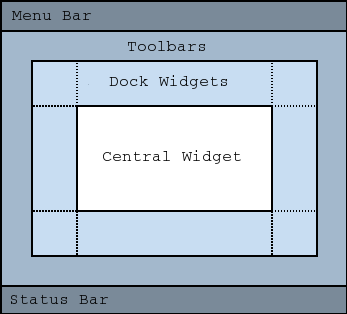
\includegraphics[width=0.5\textwidth]{mainwindowlayout}
\end{figure}

\begin{notice}
主窗口必须设置中央部件。
\end{notice}

\subsection{创建主窗口组件}

中央部件通常是标准 Qt 部件,如 QTextEdit 或 QGraphicsView,也可自定义部件。
用setCentralWidget()来设置中央部件。

主窗口可以是单文档界面或多文档界面。 
Qt 中设置 QMdiArea 为中央部件即创建了多文档界面。

下面举例说明主窗口可以添加的部件。

\subsubsection{创建菜单}

Qt 用 QMenu 类实现菜单,主窗口将其放在 QMenuBar。
可以添加 QAction 到QMenu,一个QAction代表菜单中的一个条目。

用menuBar()可以得到主窗口的菜单栏,用 QMenuBar::addMenu 添加菜单。

QMainWindow 默认有一个菜单栏,可以用setMenuBar()自定义一个新的菜单栏。
如果不想用 QMenuBar ,也可以用setMenuWidget()来定制菜单栏。

创建菜单代码示例:

\begin{lstlisting}[language=C++]
void MainWindow::createMenus()
{
    fileMenu = menuBar()->addMenu(tr("&File"));
    fileMenu->addAction(newAct);
    fileMenu->addAction(openAct);
    fileMenu->addAction(saveAct);
}
\end{lstlisting}

createPopupMenu()可以创建弹出式菜单,它会在主窗口收到 context menu 事件时弹出。
停靠部件和菜单栏默认实现了右键菜单,可以重写createPopupMenu()创建自定义菜单。

\subsubsection{创建工具栏}

Qt 用 QToolBar 类实现工具栏,可以用addToolBar()添加工具栏到主窗口。

可以设置 Qt::ToolBarArea 来控制工具栏的初始位置。可以用addToolBarBreak()或insertToolBarBreak()分割工具栏所在的区域,前者可使接下来添加的工具栏换至新的一行,后者添加了一个工具栏分隔符。用 QToolBar::setAllowedAreas 加 QToolBar::setMovable 可以限制用户放工具栏的位置。

工具栏图标的尺寸可以用iconSize()获取,它是平台相关的。可以用setIconSize()设置固定尺寸。用setToolButtonStyle()可以修改工具栏图标外观。

创建工具栏代码示例:

\begin{lstlisting}[language=C++]
void MainWindow::createToolBars()
{
    fileToolBar = addToolBar(tr("File"));
    fileToolBar->addAction(newAct);
}
\end{lstlisting}

\subsection{创建停靠部件}

Qt 用 QDockWidget 类实现停靠部件。停靠部件即可以停靠在主窗口的窗口,可以用 \hl{addDockWidget()} 添加停靠部件到主窗口。

可以设置 \hl{Qt::DockWidgetArea} 来控制停靠部件的位置,有上、下、左、右四种。\hl{setCorner()} 可以让一个角落属于某个相邻的区域。
默认情况下,一个区域只有一个停靠部件,用 \hl{setDockNestingEnabled()} 可以使其能上下或者左右排列多个停靠部件。

两个停靠部件也可以堆叠在一起,然后使用 QTabBar 来选择应显示哪个部件。

创建并添加停靠部件到主窗口的代码示例:


\begin{lstlisting}[language=C++]
QDockWidget *dockWidget = new QDockWidget(tr("Dock Widget"), this);
dockWidget->setAllowedAreas(Qt::LeftDockWidgetArea | Qt::RightDockWidgetArea);
dockWidget->setWidget(dockWidgetContents);
addDockWidget(Qt::LeftDockWidgetArea, dockWidget);
\end{lstlisting}

\subsection{状态栏}

用 \hl{setStatusBar()} 可以设置状态栏,调用 \hl{statusBar()} 会返回主窗口的状态栏。查看 QStatusBar 获取更多内容。

\subsection{存储状态}

QMainWindow 用 \hl{saveState()} 保存布局,用 \hl{restoreState()} 恢复布局。包括工具栏和停靠部件的位置和相对主窗口的尺寸。

\begin{seeAlso}
QMenuBar,QToolBar,QStatusBar, QDockWidget,Application Example,
Dock Widgets Example,MDI Example,SDI Example 和 Menus Example。
\end{seeAlso}

\section{成员变量文档}

enum QMainWindow::DockOption flags QMainWindow::DockOptions

该枚举包含指定 QMainWindow 停靠行为的标志。

\begin{tabular}{|l|l|m{25em}|}
\hline
函数	& 值	&描述 \\ 
\hline
QMainWindow::AnimatedDocks&	0x01	&同 animated 属性 \\
\hline
QMainWindow::AllowNestedDocks	&0x02&	同 dockNestingEnabled 属性 \\ 
\hline
QMainWindow::AllowTabbedDocks	&0x04	&允许形成下方有 tabBar 的重合部件 \\ 
\hline
QMainWindow::ForceTabbedDocks	&0x08&	每个停靠区域都只包含一个选项卡式停靠部件。
换句话说,停靠区域里不能上下或左右排列停靠部件。如果设置了此选项,则 AllowNestedDocks 不起作用。 \\
\hline
QMainWindow::VerticalTabs	&0x10	&设置 tabBar 在竖直左方位置(默认在下方),包含了 AllowTabbedDocks。另请参阅 setTabPosition () \\ 
\hline
QMainWindow::GroupedDragging	&0x20	&拖动停靠部件的标题栏时,将拖动所有和它在一起的停靠部件。
包含了 AllowTabbedDocks 。在某些停靠部件有区域限制时会有问题。(该枚举值在 Qt 5.6 添加) \\ 
\hline
\end{tabular}

这些选项只是控制停靠部件将如何放入 QMainWindow,不会重新排列停靠部件。
所以要先给停靠部件设置这些选项,再添加到主窗口。AnimatedDocks 和 VerticalTabs 选项例外,它们可以随后设置。

此枚举值在 Qt 4.3 引入和修改

DockOptions 是 QFlags<DockOption> 的 typedef。
它存储 DockOption 值的 OR 组合。

\section{属性文档}

animated : bool

此属性表示是否对操作停靠部件和工具栏进行动画处理

当停靠部件或工具栏在主窗口拖动时,主窗口会显示它们将停靠在什么位置。设置此属性使 QMainWindow 在平滑动画中移动其内容。清除此属性会使它们啪地进入新位置。

默认情况,此属性是生效的。如果主窗口调整尺寸或重绘太慢,可能会无效。

设置此属性与使用 setDockOptions () 设置 AnimatedDocks 选项相同。

该属性在 Qt 4.2 引入

存取函数:

\begin{tabular}{|c|c|}
\hline
    返回类型 &	函数名 \\ 
\hline
bool	& isAnimated() const \\ 
\hline
void	& setAnimated(bool enabled) \\ 
\hline
\end{tabular}

\splitLine

dockNestingEnabled : bool

此属性表示停靠部件是否可以嵌套。

如果此属性为false,停靠区域只能是水平的或垂直的一行。
如果此属性为true,停靠区域所占的区域可以沿任意方向拆分以包含更多的停靠部件。

\begin{quote}
译者注:如果设为 true,两个 dock 可以上面一块,
下面一块,显示在一个区域里,如果设为 false,
则两个 dock 只能变成选项卡式占用一个区域。
\end{quote}

只有在包含大量停靠部件的应用程序中,才需要停靠嵌套。
它给用户更大的自由来组织主窗口。但是,当停靠部件拖过主窗口时,停靠嵌套会导致更加复杂和不太直观的行为。

设置此属性与使用 setDockOptions () 设置 AllowNestedDocks 选项相同。

该属性在 Qt 4.2 引入

存取函数:

\begin{tabular}{|c|c|}
    \hline
    返回类型 &	函数名 \\ 
    \hline
    bool	& isDockNestingEnabled() const \\ 
    \hline
    void	& setDockNestingEnabled(bool enabled) \\ 
    \hline
    \end{tabular}

\splitLine

dockOptions : DockOptions

此属性表示 QMainWindow 的停靠行为

默认值是 AnimatedDocks | AllowTabbedDocks

该属性在 Qt 4.3 引入

存取函数:

\begin{tabular}{|c|c|}
    \hline
    返回类型 &	函数名 \\ 
    \hline
    QMainWindow::DockOptions &	dockOptions() const \\ 
    \hline
    void	&setDockOptions(QMainWindow::DockOptions options) \\ 
    \hline
    \end{tabular}

\splitLine

documentMode : bool

此属性决定选项卡式停靠部件的选项卡栏是否为文档模式。

默认为 false

该属性在 Qt 4.5 引入

存取函数:

\begin{tabular}{|c|c|}
    \hline
    返回类型 &	函数名 \\ 
    \hline
    bool&	documentMode() const \\ 
    \hline
    void&	setDocumentMode(bool enabled) \\ 
    \hline
    \end{tabular}

\begin{seeAlso}
QTabBar::documentMode
\end{seeAlso}

\splitLine

iconSize : QSize

主窗口工具栏图标的尺寸。

默认是 GUI 样式的默认工具栏图标大小。

\begin{notice}
使用的图标必须至少具有此大小,因为图标只会缩小。
\end{notice}

存取函数:

\begin{tabular}{|c|c|}
    \hline
    返回类型 &	函数名 \\ 
    \hline 
    QSize	&iconSize() const \\ 
    \hline
    void&	setIconSize(const QSize \&iconSize) \\
    \hline
    \end{tabular}

\splitLine

tabShape : QTabWidget::TabShape

此属性表示选项卡式停靠部件的选项卡形状。

默认是 QTabWidget::Rounded

该属性在 Qt 4.5 引入

存取函数:

\begin{tabular}{|c|c|}
    \hline
    返回类型 &	函数名 \\ 
    \hline  
    QTabWidget::TabShape &	tabShape() const \\ 
    \hline
    void 	& setTabShape(QTabWidget::TabShape tabShape) \\ 
    \hline
    \end{tabular}


\begin{seeAlso}
setTabPosition ()
\end{seeAlso}

\splitLine

toolButtonStyle : Qt::ToolButtonStyle

主窗口的工具栏按钮样式。

若要使工具按钮的样式遵循系统设置,请将此属性设置为 Qt::ToolButtonFollowStyle。
在 Unix 上,将使用桌面环境变量中的用户设置。在其他平台上,Qt::ToolButtonFollowStyle 意思是仅显示图标。

默认是 Qt::ToolButtonIconOnly

存取函数:

\begin{tabular}{|c|c|}
    \hline
    返回类型 &	函数名 \\ 
    \hline  
    Qt::ToolButtonStyle &	toolButtonStyle() const \\ 
    \hline
    void 	& setToolButtonStyle(Qt::ToolButtonStyle toolButtonStyle) \\ 
    \hline
    \end{tabular}

\splitLine

unifiedTitleAndToolBarOnMac : bool

此属性表示窗口是否使用 macOS 上的统一标题和工具栏外观

请注意,与 Qt 4 相比,Qt 5 实现有几个限制:

\begin{compactitem}
\item 不支持在包含 OpenGL 内容的窗口中使用。这包括 QGLWidget 和 QOpenGLWidget。
\item 使用可停靠或可移动工具栏可能会导致绘制错误,不建议使用。
\end{compactitem}

该属性在 Qt 5.2 引入

存取函数:

\begin{tabular}{|c|c|}
    \hline
    返回类型 &	函数名 \\ 
    \hline  
    bool  &	unifiedTitleAndToolBarOnMac() const \\ 
    \hline
    void  &	setUnifiedTitleAndToolBarOnMac(bool set) \\ 
    \hline
    \end{tabular}

\section{成员函数文档}


QMainWindow::QMainWindow(QWidget *parent = nullptr, Qt::WindowFlags flags = Qt::WindowFlags())

主窗口构造函数,指定 parent 和 flags

主窗口设置了 Qt::Window 标志,因此它总作为顶层窗口被创建。

\splitLine

[signal]void QMainWindow::iconSizeChanged(const QSize \&iconSize)

当窗口图标被改变时,将发出此信号。新图标的尺寸为 iconSize。

您可以将此信号连接到其他组件,以帮助保持应用程序的一致外观。

\begin{seeAlso}
setIconSize ().
\end{seeAlso}

\splitLine

[signal]void QMainWindow::tabifiedDockWidgetActivated(QDockWidget *dockWidget)

当通过选择选项卡激活停靠部件时,将发出此信号。 dockWidget 表示激活的停靠部件。

该函数在 Qt 5.8 引入

\begin{seeAlso}
tabifyDockWidget() and tabifiedDockWidgets()。
\end{seeAlso}

\splitLine

[signal]void QMainWindow::toolButtonStyleChanged(Qt::ToolButtonStyle toolButtonStyle)

当窗口的工具栏按钮样式更改时,将发出此信号。toolButtonStyle 表示新样式。

您可以将此信号连接到其他组件,以帮助保持应用程序的一致外观。

\begin{seeAlso}
setToolButtonStyle ()
\end{seeAlso}

\splitLine

[virtual]QMainWindow::$\sim$QMainWindow()

销毁主窗口

\splitLine

void QMainWindow::addDockWidget(Qt::DockWidgetArea area, 
    QDockWidget *dockwidget)

添加指定 dockwidget 到指定 area.

\splitLine

void QMainWindow::addDockWidget(Qt::DockWidgetArea area, QDockWidget *dockwidget, Qt::Orientation orientation)

将 dockwidget 添加到指定的 area,方向由 orientation 指定。

\splitLine

void QMainWindow::addToolBar(Qt::ToolBarArea area, QToolBar *toolbar)

在主窗口中将 toolbar 添加到指定的 area。toolbar 放置在当前工具栏块(比如分隔符)的后面。如果主窗口已管理 toolbar,则只会将工具栏移动到 area。


\begin{seeAlso}
insertToolBar (),addToolBarBreak () 和 insertToolBarBreak ()
\end{seeAlso}

\splitLine

void QMainWindow::addToolBar(QToolBar *toolbar)

这是一个重载函数。

相当于调用 addToolBar(Qt::TopToolBarArea, toolbar)

\splitLine

QToolBar *QMainWindow::addToolBar(const QString \&title)

这是一个重载函数。

创建 QToolBar 的一个对象,设置它的窗口标题为 title 并将它添加到上方的工具栏区域。

\begin{seeAlso}
setWindowTitle ()
\end{seeAlso}

\splitLine

void QMainWindow::addToolBarBreak(Qt::ToolBarArea area = Qt::TopToolBarArea)

添加一个工具栏 break。这时,新添加的工具条将不再紧跟前一个工具条,而是另起一行。

\splitLine

QWidget *QMainWindow::centralWidget() const

返回主窗口的中央部件。如果尚未设置中央部件,则此函数返回零。

\begin{seeAlso}
setCentralWidget ()
\end{seeAlso}

\splitLine

[override virtual protected]void QMainWindow::contextMenuEvent(QContextMenuEvent \emph{*event})

重写:QWidget::contextMenuEvent (QContextMenuEvent *event)

Qt::DockWidgetArea QMainWindow::corner(Qt::Corner corner) const

返回占用指定 corner 的停靠部件区域。

\begin{seeAlso}
setCorner ()
\end{seeAlso}

\splitLine

[virtual]QMenu *QMainWindow::createPopupMenu()

返回一个弹出式菜单,其中包含主窗口中存在的工具栏和停靠部件的可选中条目。如果没有工具栏和停靠小部件,则此函数将返回nullptr。

默认情况下,当用户激活上下文菜单时,主窗口会调用此函数,通常通过右键单击工具栏或停靠部件。

如果要创建自定义弹出式菜单,请重新实现此功能并返回新创建的弹出式菜单。
弹出式菜单的所有权将传输到调用方。

\begin{seeAlso}
addDockWidget (),addToolBar () 和 menuBar ()
    \end{seeAlso}
    
\splitLine

Qt::DockWidgetArea QMainWindow::dockWidgetArea(QDockWidget \emph{*dockwidget}) const

返回 dockwidget 的 Qt::DockWidgetArea。如果 dockwidget 没有被加入主窗口,此函数返回Qt::NoDockWidgetArea

\begin{seeAlso}
addDockWidget (),splitDockWidget () 和 Qt::DockWidgetArea
\end{seeAlso}

\splitLine

[override virtual protected]bool QMainWindow::event(QEvent \emph{*event})

重写:QWidget::event (QEvent *event)

\splitLine

void QMainWindow::insertToolBar(QToolBar \emph{*before}, QToolBar \emph{*toolbar})

将 toolbar 插入到 before 工具栏占用的区域之前。
例如,在正常的从左到右布局操作中,toolbar 将显示在水平工具栏区域中 before 工具栏的左侧。

\begin{seeAlso}
insertToolBarBreak (),addToolBar () 和 addToolBarBreak ()
\end{seeAlso}

\splitLine

void QMainWindow::insertToolBarBreak(QToolBar \emph{*before})

在 before 工具栏左侧插入一个工具栏 break。

\splitLine

QMenuBar *QMainWindow::menuBar() const

返回主窗口的菜单栏。如果菜单栏不存在,则此函数将创建并返回一个空菜单栏。

如果希望 Mac 应用程序中的所有窗口共享一个菜单栏,请不要使用此函数来创建它,
因为此处创建的菜单栏将把 QMainWindow 作为它的父对象。
必须创建一个没有父对象的菜单栏,然后可以在所有 Mac 窗口之间共享该菜单栏。

这样创建:

\begin{lstlisting}[language=C++]
QMenuBar *menuBar = new QMenuBar(nullptr);
\end{lstlisting}

\begin{seeAlso}
setMenuBar()
\end{seeAlso}

\splitLine

QWidget *QMainWindow::menuWidget() const

返回主窗口的菜单栏。如果尚未构造菜单栏,返回 null。

该函数在 Qt 4.2 引入

\begin{seeAlso}
setMenuWidget ()
\end{seeAlso}

\splitLine

void QMainWindow::removeDockWidget(QDockWidget \emph{*dockwidget})

从主窗口布局中移除 dockwidget 并将其隐藏。注意,dockwidget 没有被 delete。

\splitLine

void QMainWindow::removeToolBar(QToolBar \emph{*toolbar})

从主窗口布局中移除 toolbar 并将其隐藏。注意,toolbar 没有被 delete。

\splitLine

void QMainWindow::removeToolBarBreak(QToolBar \emph{*before})

删除 before 工具栏之前的一个工具栏 break。

\splitLine

void QMainWindow::resizeDocks(const QList<QDockWidget *> \emph{\&docks},
 const QList<int> \emph{\&sizes}, Qt::Orientation \emph{orientation})

将 \emph{docks} 列表中的停靠部件调整为 \emph{sizes} 列表中的相应尺寸(以像素为单位)。如果 orientation 为 Qt::Horizontal,则调整宽度,否则调整高度。尺寸会调整,以遵守设置的最大尺寸和最小尺寸,并且 QMainWindow 本身不会调整大小。任何多余或缺少的空间将根据尺寸的相对权重分布在部件之间。

示例:

\begin{lstlisting}[language=C++]
resizeDocks({blueWidget, yellowWidget}, {20 , 40}, Qt::Horizontal);
\end{lstlisting}


如果蓝色和黄色部件嵌套在同一级别上,它们将被调整大小,使黄色部件是蓝色部件的两倍大

如果某些部件在选项卡中分组,则每个组只应指定一个部件。不在列表中的部件可能会改变以遵守约束。

该函数在 Qt 5.6 引入

\splitLine

bool QMainWindow::restoreDockWidget(QDockWidget \emph{*dockwidget})

如果在调用 restoreState () 后创建 \emph{dockwidget} 的状态,则恢复状态。
如果状态已恢复,则返回true;否则返回false。

\begin{seeAlso}
restoreState() 和 saveState()
\end{seeAlso}

\splitLine

bool QMainWindow::restoreState(const QByteArray \emph{\&state}, int version = 0)

还原主窗口工具栏和停靠部件的 \emph{state}。也恢复 corner 的设置。
version 编号与存储在 state 中的号码进行比较。
如果它们不匹配,主窗口的状态保持不变,并且函数将返回false;否则,状态将恢复,函数返回 true。

若要恢复用 QSettings 保存的窗口 geometry,可以这么写:

\begin{lstlisting}[language=C++]
void MainWindow::readSettings()
{
    QSettings settings("MyCompany", "MyApp");
    restoreGeometry(settings.value("myWidget/geometry").toByteArray());
    restoreState(settings.value("myWidget/windowState").toByteArray());
}
\end{lstlisting}

\begin{seeAlso}
saveState(),QWidget::saveGeometry(),QWidget::restoreGeometry() 和 restoreDockWidget()
\end{seeAlso}

\splitLine

QByteArray QMainWindow::saveState(int version = 0) const

保存主窗口工具栏和停靠部件的当前状态。这包括用 setCorner() 设置的角落区域。
version 作为数据的一部分存储。

objectName 属性用于标识每个 QToolBar 和 QDockWidget。

您应该确保此属性对于添加到 QMainWindow 的每个 QToolBar 和 QDockWidget 是唯一的。

要还原保存的状态,请传递返回值和 version 给 restoreState()。

若要在窗口关闭时保存 geometry,可以这样实现关闭事件:

\begin{lstlisting}[language=C++]
void MyMainWindow::closeEvent(QCloseEvent *event)
{
    QSettings settings("MyCompany", "MyApp");
    settings.setValue("geometry", saveGeometry());
    settings.setValue("windowState", saveState());
    QMainWindow::closeEvent(event);
}
\end{lstlisting}

\begin{seeAlso}
restoreState(), QWidget::saveGeometry() 和 QWidget::restoreGeometry()
\end{seeAlso}

\splitLine

void QMainWindow::setCentralWidget(QWidget \emph{*widget})

将主窗口的中央部件设置为 \emph{widget}。

\begin{notice}
QMainWindow 拥有 widget 指针的所有权,会在适当的时间将其删除。
\end{notice}

\begin{seeAlso}
centralWidget()
\end{seeAlso}

\splitLine

void QMainWindow::setCorner(Qt::Corner \emph{corner}, Qt::DockWidgetArea \emph{area})

用停靠部件 area 占据指定的 corner。

\begin{seeAlso}
corner()
 \end{seeAlso}

\splitLine

void QMainWindow::setMenuBar(QMenuBar \emph{*menuBar})

将主窗口的菜单栏设置为 menuBar。

\begin{notice}
QMainWindow 拥有 menuBar 指针的所有权,会在适当的时间将其删除。\end{notice}

\begin{seeAlso}
menuBar()
\end{seeAlso}

\splitLine

void QMainWindow::setMenuWidget(QWidget \emph{*menuBar})

将主窗口的菜单栏设置为 \emph{menuBar}。

QMainWindow 拥有 \emph{menuBar} 指针的所有权,会在适当的时间将其删除。

该函数在 Qt 4.2 引入

\begin{seeAlso}
menuWidget()
\end{seeAlso}

\splitLine

void QMainWindow::setStatusBar(QStatusBar \emph{*statusbar})

将主窗口的状态栏设置为 statusbar。

将状态栏设置为nullptr会将其从主窗口中删除。请注意,QMainWindow 拥有 statusbar 指针的所有权,会在适当的时间将其删除。

\begin{seeAlso}
statusBar()
\end{seeAlso}

\splitLine

void QMainWindow::setTabPosition(Qt::DockWidgetAreas \emph{areas}, QTabWidget::TabPosition \emph{tabPosition})

将停靠部件 areas 的选项卡位置设置为指定的 tabPosition。默认情况下,所有停靠区域在底部显示其选项卡。

\begin{notice}
VerticalTabs 会覆盖此方法设置的选项卡位置
\end{notice}

该函数在 Qt 4.5 引入

\begin{seeAlso}
tabPosition() 和 setTabShape()
\end{seeAlso}

\splitLine

void QMainWindow::splitDockWidget(QDockWidget \emph{*first}, QDockWidget \emph{*second}, Qt::Orientation \emph{orientation})

分割停靠部件 first 为两个停靠部件,第一个部件指针传给 first,第二个部件指针传给 second。

orientation 指定了空间的划分。Qt::Horizontal 左右分割;

Qt::Vertical 上下分割。

\begin{notice}
如果 first 位于选项卡式停靠区域中,则 second 将添加为新选项卡,这是因为单个选项卡只能包含一个停靠部件。
    \end{notice}

\begin{notice}
Qt::LayoutDirection 会影响两个分割区域的停靠部件顺序。启用从右到左布局方向时,将反转停靠部件的位置。
\end{notice}


\begin{seeAlso}
tabifyDockWidget(), addDockWidget() 和 removeDockWidget()
\end{seeAlso}

\splitLine

QStatusBar *QMainWindow::statusBar() const

返回主窗口的状态栏。如果状态栏不存在,则此函数将创建并返回一个空状态栏。

\begin{seeAlso}
setStatusBar()
\end{seeAlso}

\splitLine

QTabWidget::TabPosition QMainWindow::tabPosition(Qt::DockWidgetArea \emph{area}) const

返回停靠区域 area 的位置。

\begin{notice}
如果设置了 VerticalTabs ,会覆盖此函数的返回值。
\end{notice}

该函数在 Qt 4.5 引入

\begin{seeAlso}
setTabPosition() 和 tabShape()
\end{seeAlso}

\splitLine

QList<QDockWidget *> QMainWindow::tabifiedDockWidgets(QDockWidget \emph{*dockwidget}) const

返回 \emph{dockwidget} 内堆叠着的停靠部件。

该函数在 Qt 4.5 引入

\begin{seeAlso}
tabifyDockWidget ()
\end{seeAlso}

\splitLine

void QMainWindow::tabifyDockWidget(QDockWidget \emph{*first}, QDockWidget \emph{*second})

将 \emph{second} 停靠部件移动到 \emph{first} 停靠部件旁形成一个选项卡式停靠区域。

\begin{seeAlso}
tabifiedDockWidgets()
\end{seeAlso}

\splitLine

QWidget *QMainWindow::takeCentralWidget()

从主窗口中移除中央部件。

返回中央部件的指针。

该函数在 Qt 5.2 引入

\splitLine

Qt::ToolBarArea QMainWindow::toolBarArea(QToolBar \emph{*toolbar}) const

返回 toolbar 的 Qt::ToolBarArea。
 如果主窗口没有添加 toolbar ,返回 Qt::NoToolBarArea。

\begin{seeAlso}
addToolBar(), addToolBarBreak() 和 Qt::ToolBarArea
\end{seeAlso}

\splitLine

bool QMainWindow::toolBarBreak(QToolBar \emph{*toolbar}) const

返回 \emph{toolbar} 之前是否有工具栏 break。

\begin{seeAlso}
addToolBarBreak() 和 insertToolBarBreak()
    \end{seeAlso}